\documentclass[a4paper]{scrartcl}
\usepackage[utf8]{inputenc}  
\usepackage[T1]{fontenc}
\usepackage{lmodern}           
\usepackage[ngerman]{babel}

% Was wir vielleicht brauchen koennten:
%\usepackage{amsmath} % More math.
%\usepackage[perpage,bottom]{footmisc} % Footnote configuration.

% Was wir ziemlich sicher brauchen:
\usepackage{fancyhdr} % For header and footer format
%\usepackage{fancyref} % For fancy references
\usepackage{listings} % For code listings
\usepackage{booktabs} % For tables
\usepackage[perpage,bottom]{footmisc} % Footnote configuration
\usepackage{graphicx} % For includegraphics
\usepackage[page,titletoc]{appendix} % For appendix in toc
\usepackage{color} % For colors, not sure if I truly need it anymore
\usepackage{caption} % For nicer listing captions
\usepackage{lipsum} % For blindtext (use \lipsum)
\usepackage{xspace} % For horizontal space.

% Bald wieder loeschen:
\usepackage{lipsum}

% Keine Ahnung warum, aber "`bla"' funktioniert bei mir nicht.
\newcommand{\enquote}[1]{\glqq{}#1\grqq{}}

% Hyperref macht Links hinter die Sections und manipuliert PDF-Metadaten:
\usepackage[
colorlinks=false,
pdfborder={0 0 0},
pdftitle={Zufällige Polygone und kürzeste Wege},
pdfsubject={Abschlussbericht zum Softwareprojekt \enquote{Zufällige Polygone und kürzeste Wege}},
pdfauthor={Steve Dierker, Marcel Ehrhardt, Jannis Ihrig, Malte Rohde, Sebastian Thobe, Kadir Tugan}
%pdfkeywords={}
]{hyperref}

% Pimp my listings environment.
% Credits go to stackoverflow:
% http://stackoverflow.com/questions/741985/latex-source-code-listing-like-in-professional-books
\lstset{
         basicstyle=\footnotesize\ttfamily, % Standardschrift
         numberstyle=\tiny,          % Stil der Zeilennummern
         numbers=left,
         stepnumber=1,
         numbersep=7pt,              % Abstand der Nummern zum Text
         keywordstyle=\bfseries\ttfamily,
         tabsize=2,                  % Groesse von Tabs
         extendedchars=true,         %
         breaklines=true,            % Zeilen werden Umgebrochen       
         showspaces=false,           % Leerzeichen anzeigen ?
         showtabs=false,             % Tabs anzeigen ?
         %frame=b,                   % Linie unten
         breakatwhitespace=true,
         xleftmargin=17pt,
         framexleftmargin=17pt,
         framexrightmargin=5pt,
         framexbottommargin=4pt,
         showstringspaces=false      % Leerzeichen in Strings anzeigen ?      
 }

% Pimp my captions.
\DeclareCaptionFont{white}{\color{white}}
\DeclareCaptionFormat{listing}{\colorbox[cmyk]{0.43, 0.35, 0.35,0.01}{\parbox{\textwidth}{\hspace{15pt}#1#2#3}}}
\captionsetup[lstlisting]{format=listing,labelfont=white,textfont=white, singlelinecheck=false, margin=0pt, font={bf}}
%\DeclareCaptionFormat{figure}{\colorbox[cmyk]{0.43, 0.35, 0.35,0.01}{\parbox{\textwidth}{\hspace{15pt}#1#2#3}}}
%\captionsetup[figure]{format=listing,labelfont=white,textfont=white, singlelinecheck=false, margin=0pt, font={bf,footnotesize}}
%\DeclareCaptionFormat{table}{\colorbox[cmyk]{0.43, 0.35, 0.35,0.01}{\parbox{\textwidth}{\hspace{15pt}#1#2#3}}}
%\captionsetup[table]{format=listing,labelfont=white,textfont=white, singlelinecheck=false, margin=0pt, font={bf,footnotesize}}

% Listing environment for C
\lstnewenvironment{code}[1][]
  {\minipage{\linewidth} 
   \lstset{language=C,#1}}
  {\endminipage}

% Konfiguration der Titelseite:
\title{
{\normalsize Softwareprojekt über Anwendung effizienter Algorithmen\\ Wintersemester 2011/12}
\\[4ex] 
{\Large Abschlussbericht zum Softwareprojekt\\ \enquote{Zufällige Polygone und kürzeste Wege}}
\\[6ex]
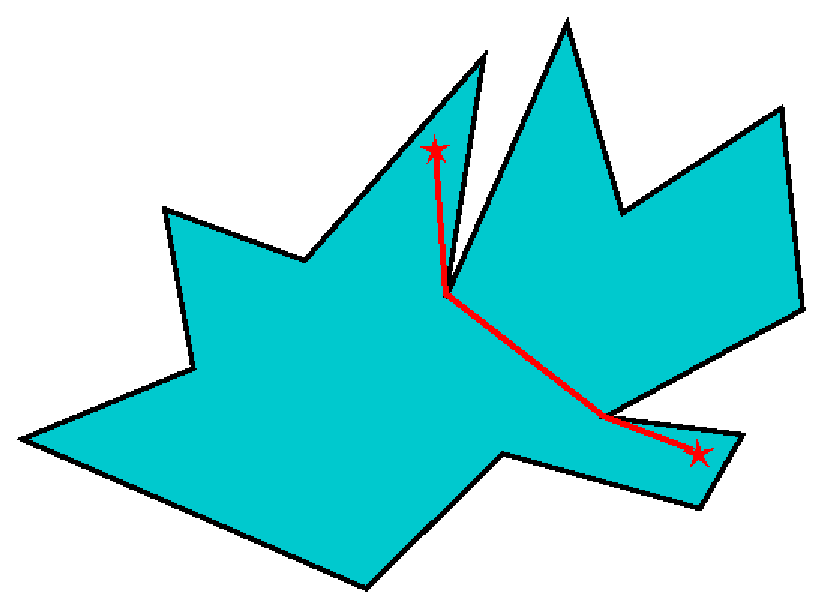
\includegraphics[width=0.4\textwidth]{img/polygons}
\\[3.5cm]}
\author{Steve Dierker \and Marcel Ehrhardt \and Jannis Ihrig \and Malte Rohde \and Sebastian Thobe \and Kadir Tugan}

\date{\vspace{2.5cm} \today{}}

\begin{document}

\begin{titlepage}
\pagenumbering{alph}
\maketitle
\thispagestyle{empty}
\vfill{}
\end{titlepage}

\pagestyle{empty}
\pagenumbering{roman}
%\include{parts/abstract}
\tableofcontents
\clearpage

\pagenumbering{arabic}
\pagestyle{fancy}
\setcounter{page}{1}

% Hier hin unsere Kapitel.
\section{Test-Kapitel}

Wir zitieren mal fröhlich einfach Mr. Rote~\cite{asano11shortestpath}. Hat funktioniert. Und nun noch ein bisschen Text.
\lipsum
\lipsum

\section{Einleitung}

  Die algorithmische Geometrie als Teilgebiet der Informatik beschäftigt sich
  mit der algorithmischen Lösung geometrischer Probleme. Einfache Polygone
  (überschneidungsfreie, zusammenhängende, planare Vielecke) bilden die
  Grundlage vieler Aufgabengebiete der algorithmischen Geometrie. Als
  naheliegendes Beispiel bezeichnet die Triangulierung die Zerlegung eines
  Polygons in eine Menge von Dreiecken, die die Fläche des Polygons
  überdecken. Diese Dreieckszerlegung ermöglicht die Lösung einer ganzen Reihe
  weiterer geometrische Probleme.

  Zum Testen und zur Evaluation polygon-basierter geometrischer
  Algorithmen ist es oft von Vorteil, über eine beliebige Menge einfacher
  Polygone zu verfügen, wobei diese, um eine gewisse Aussagekraft der
  Experimente zu gewährleisten, möglichst alle (in einem
  definierten planaren Raum) vorstellbaren Polygone erzeugen können sollten. Die
  massenweise Erzeugung solcher \emph{zufälliger Polygone} ist ein
  Forschungsgebiet, dem in den vergangenen Jahrzehnten daher vermehrt
  wissenschaftliche Aufmerksamkeit zugekommen ist. Die entstandenen
  Lösungswege und Algorithmen unterscheiden sich unter anderem in ihrer
  Komplexität, im Speicherverbrauch sowie in der Art und
  \enquote{Zufälligkeit} der erzeugten Polygone.

  Der vorliegende Text ist der Abschlussbericht des Softwareprojekts
  \emph{Zufällige Polygone und kürzeste Wege}, welches im Rahmen des Moduls
  \enquote{Softwareprojekt: Anwendung von Algorithmen} unter Leitung von Prof.
  Dr. Günter Rote durchgeführt wurde. Das Ziel des Projekts war die
  Entwicklung einer Softwarebibliothek, welche über verschiedenene Algorithmen
  zur Erzeugung zufälliger Polygone verfügen und diese unter anderem
  über eine grafische Schnittstelle dem Benutzer zur Verfügung stellen sollte.
  Das Projekt wurde mit Ende des Wintersemesters 2011/2012 abgeschlossen.

  Im Folgenden werden wir zunächst die Zielsetzung des Projekts, funktionale
  und nicht-funktionale Anforderungen an die zu implementierende Software,
  sowie Einschränkungen der Zielsetzung darstellen. Anschließend erfolgt eine
  kurze Erläuterung des von uns gewählten Entwicklungsprozesses und dessen
  Umsetzung. Im Hauptteil des Berichts gehen wir detailliert auf die
  Eigenschaften der einzelnen Algorithmen sowie auf die während der
  Entwicklung aufgetretenden Probleme und deren Lösungen ein. In
  Kapitel~\ref{sec:manual} findet der Leser einen umfassenden
  \emph{Benutzerleitfaden} für die entstandene Softwarelösung. Im letzten
  Kapitel schließen wir den Bericht mit einem kurzen Fazit zum Projektablauf
  sowie zu unserer Einschätzung der Brauchbarkeit der Software.


\cleardoublepage
\phantomsection

% Bibliography
\addcontentsline{toc}{section}{Literatur}
\bibliographystyle{alpha}
\bibliography{report}

\end{document}
